\section{Results}
\label{sec:results}



\begin{figure*}
\begin{tabular}{ l l l}
  \hspace{2.0cm}(a) & \hspace{4.2cm}(b) & \hspace{4.2cm}(c) \\
\end{tabular}\\
\resizebox{6in}{!}{
  \begin{tabular}{ c c c}
  \hspace{-0.9cm}
  
\includegraphics[trim={4.7cm 0 1.9cm 0},clip]{figures/ndcg_ratings_num.pdf} 
  &  
  \hspace{-0.9cm}
  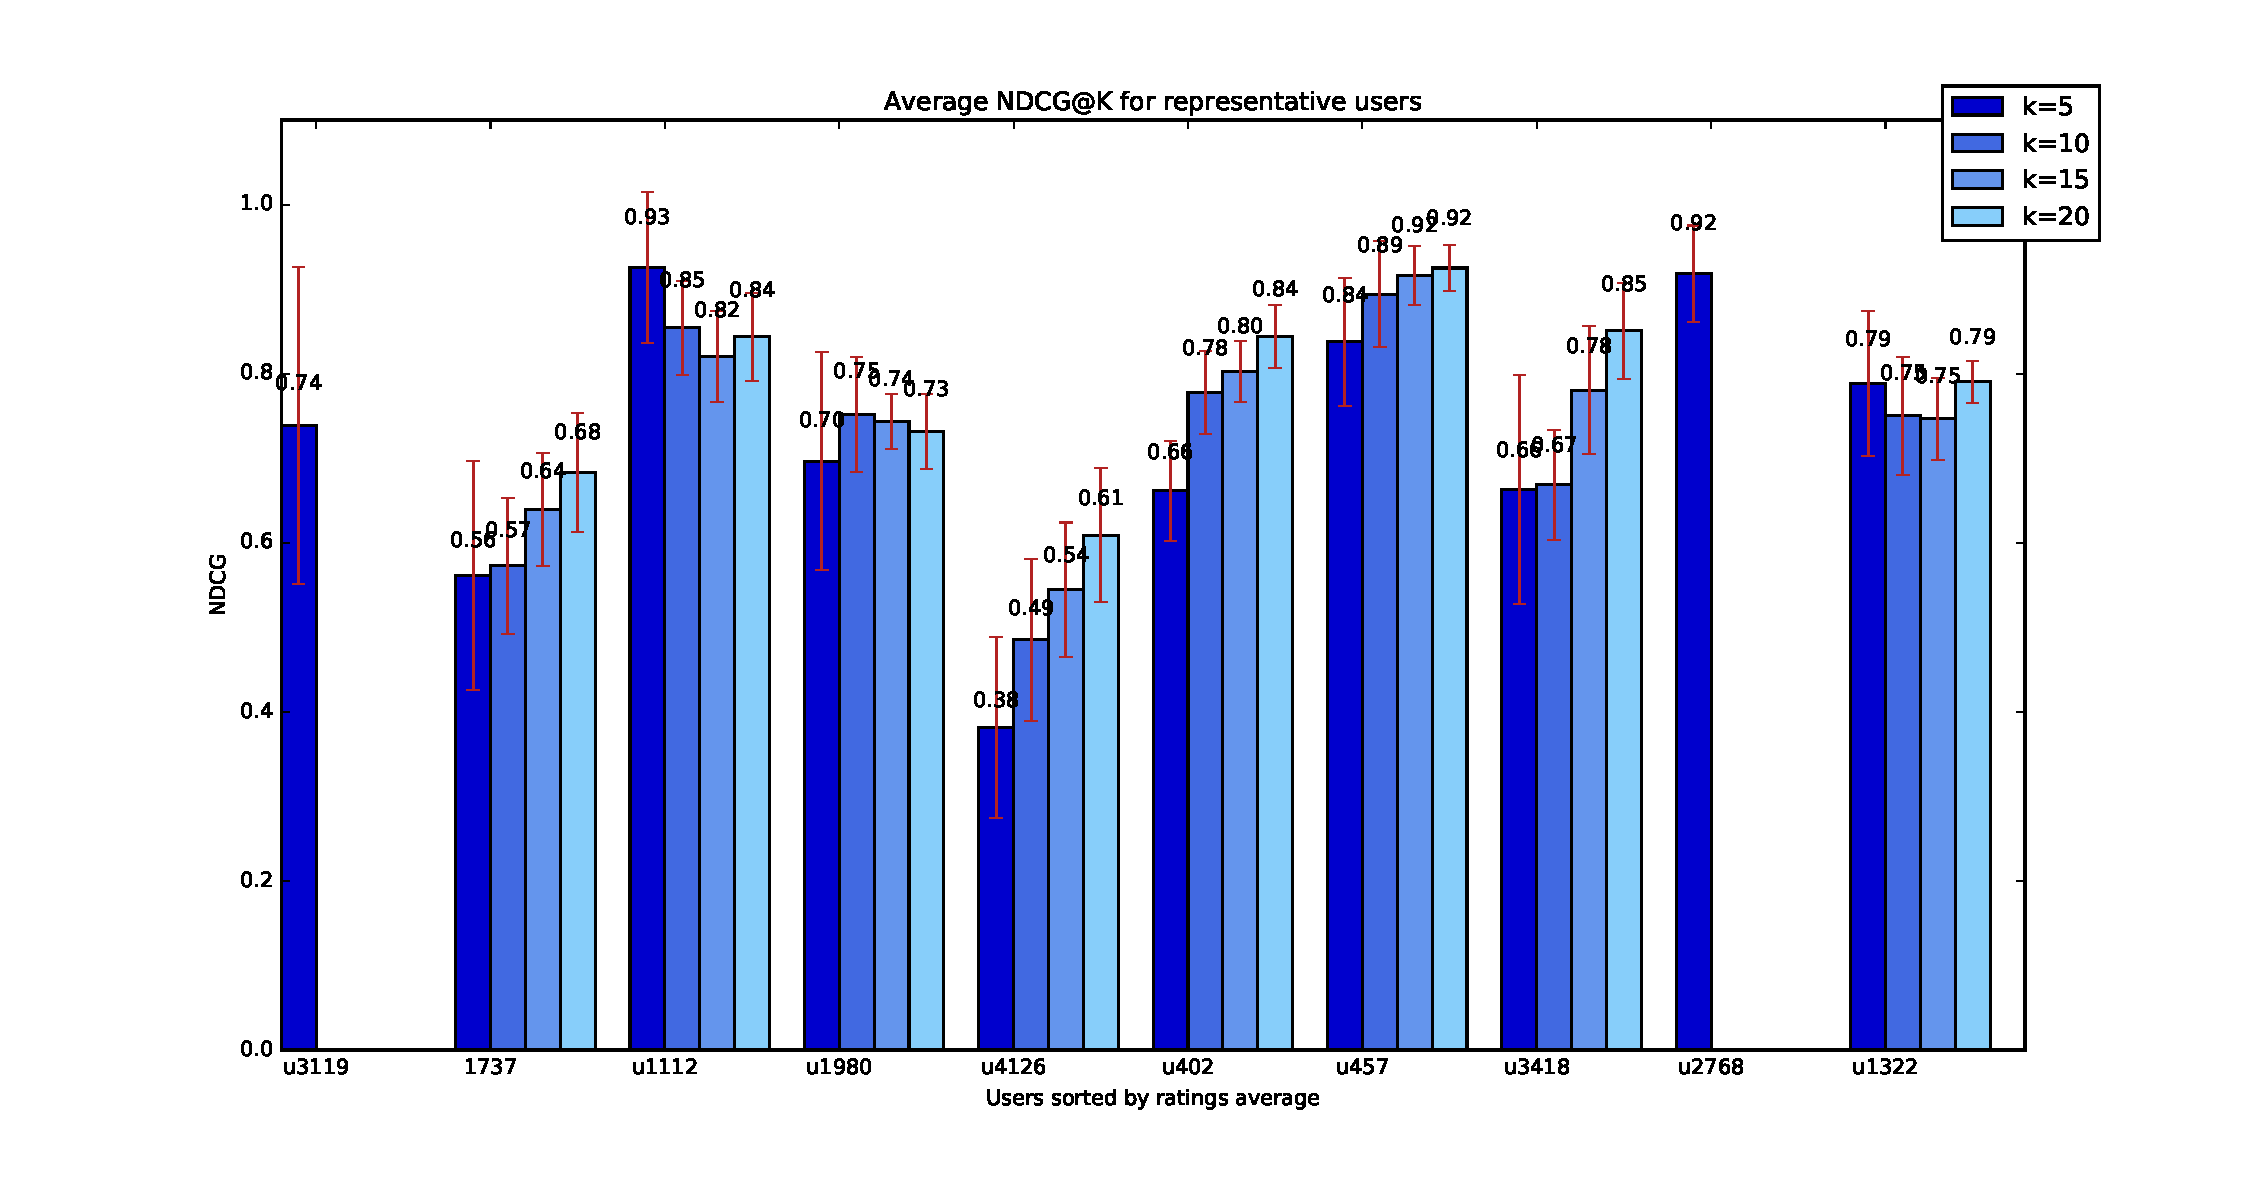
\includegraphics[trim={4.7cm 0 1.9cm 0},clip]{figures/ndcg_ratings_avg.pdf} 
  &
  \hspace{-0.9cm}
  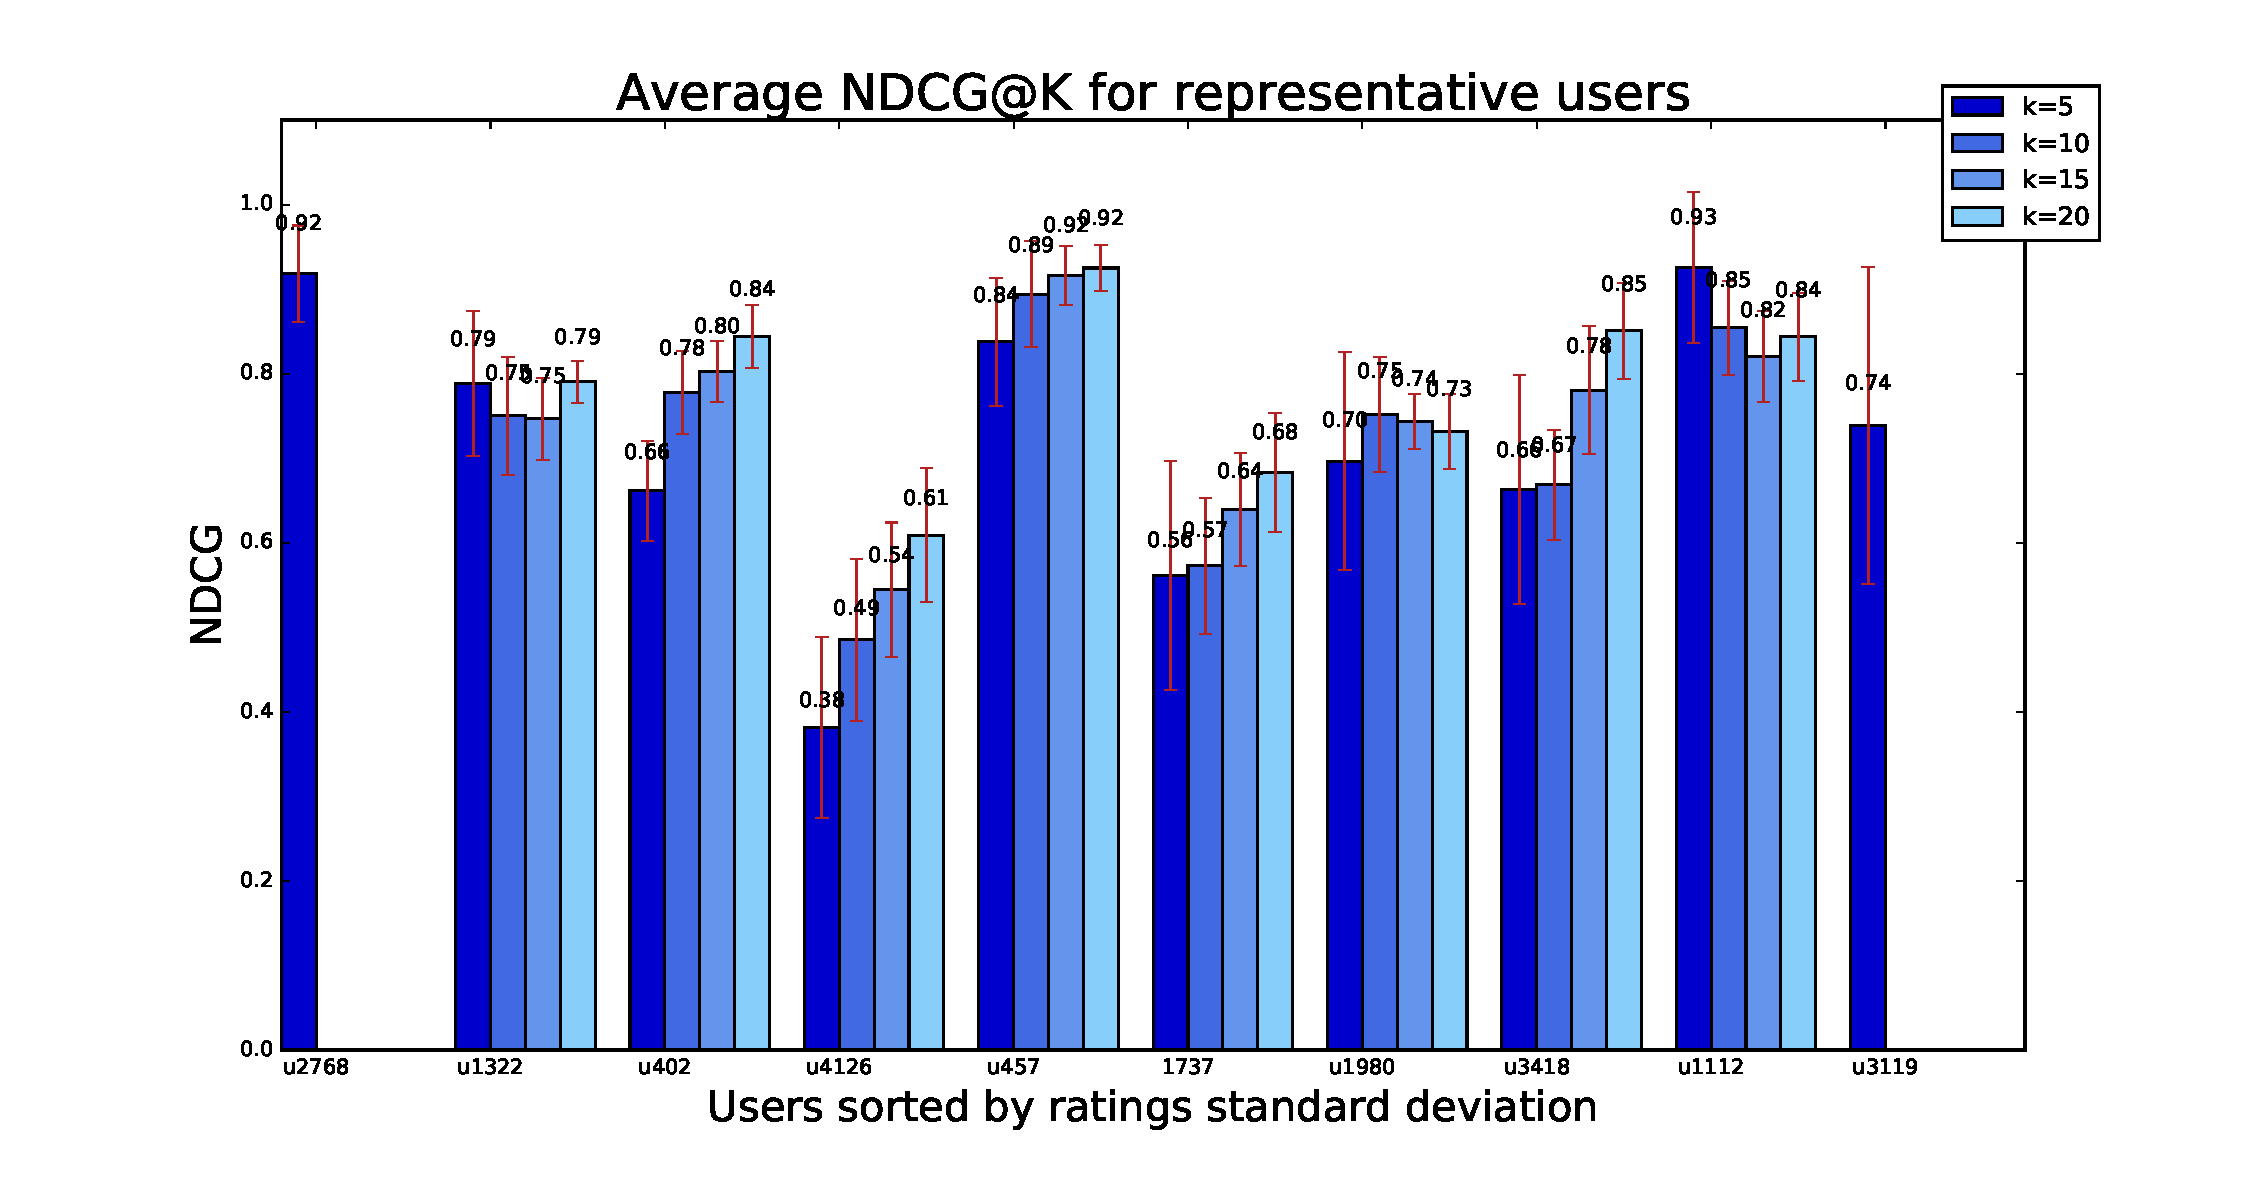
\includegraphics[trim={4.7cm 0 1.9cm 0},clip]{figures/ndcg_ratings_std.pdf} \\
\end{tabular}
}
\caption{Clustering Figure \hl{TODO better description}: 
\\(a) representative users sorted by number of ratings, (b) representative users sorted by average rating, (c) representative users sorted by rating deviation}
\label{fig:ndcg}  
\end{figure*}


\begin{figure}
\center
\resizebox{5in}{!}{
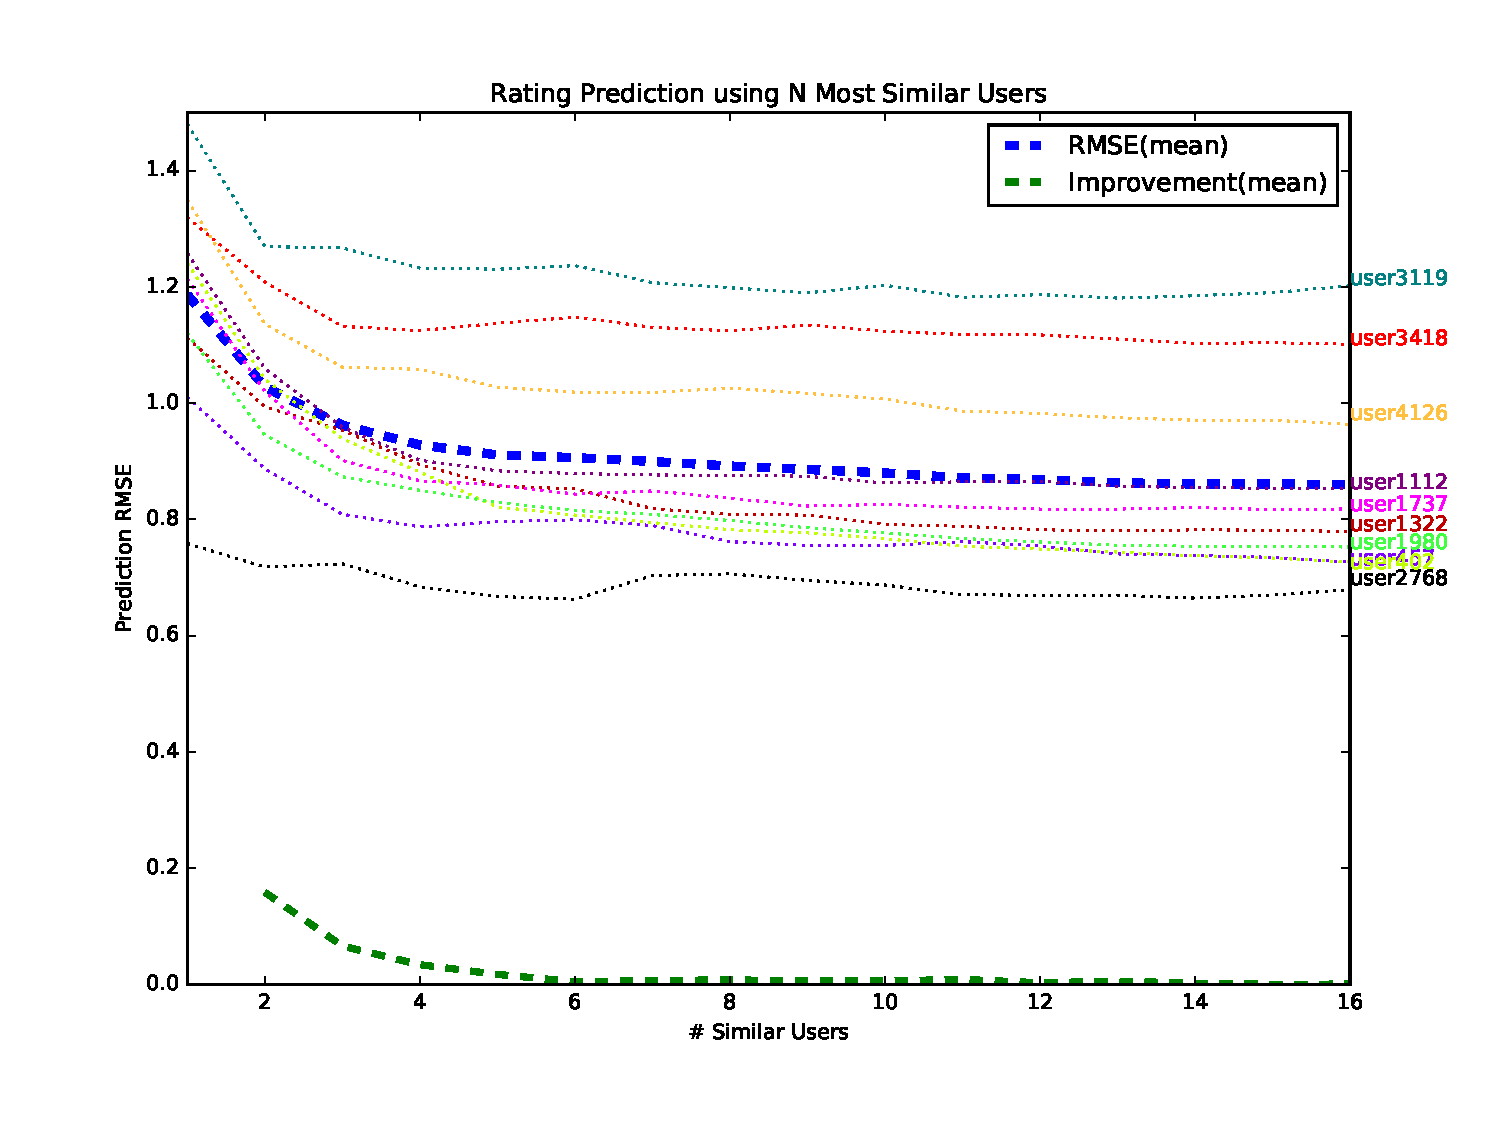
\includegraphics{figures/user_similarity.pdf} 
}
\caption{User Similarity Rating Prediction Results (RMSE vs. \# similar users)}
\label{fig:user_similarity}  
\end{figure}




\begin{figure*}
\begin{tabular}{ l l}
  \hspace{3.5cm}(a) & \hspace{7cm}(b)\\
\end{tabular}\\
\resizebox{6in}{!}{
  \begin{tabular}{c c}
  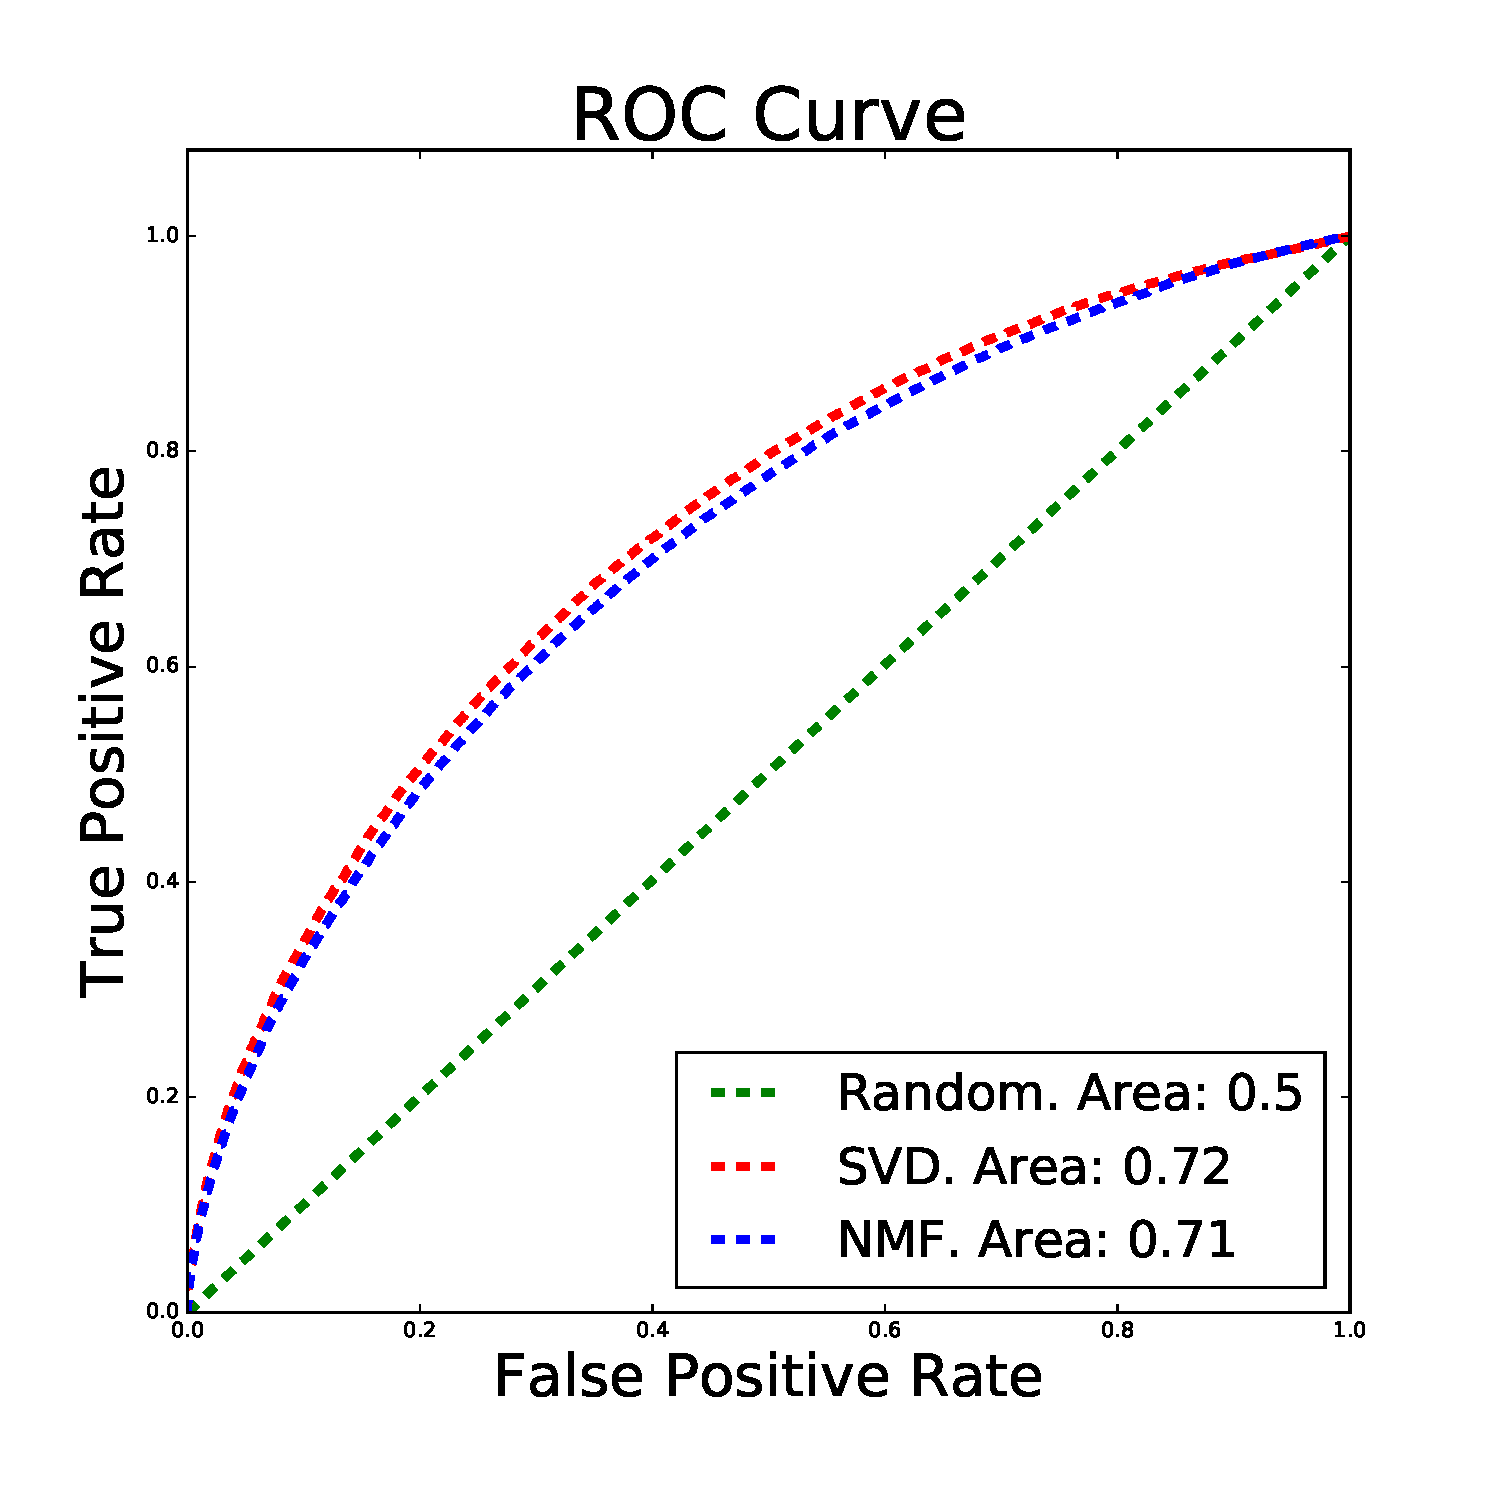
\includegraphics{figures/roc_curve.pdf} 
  &  
  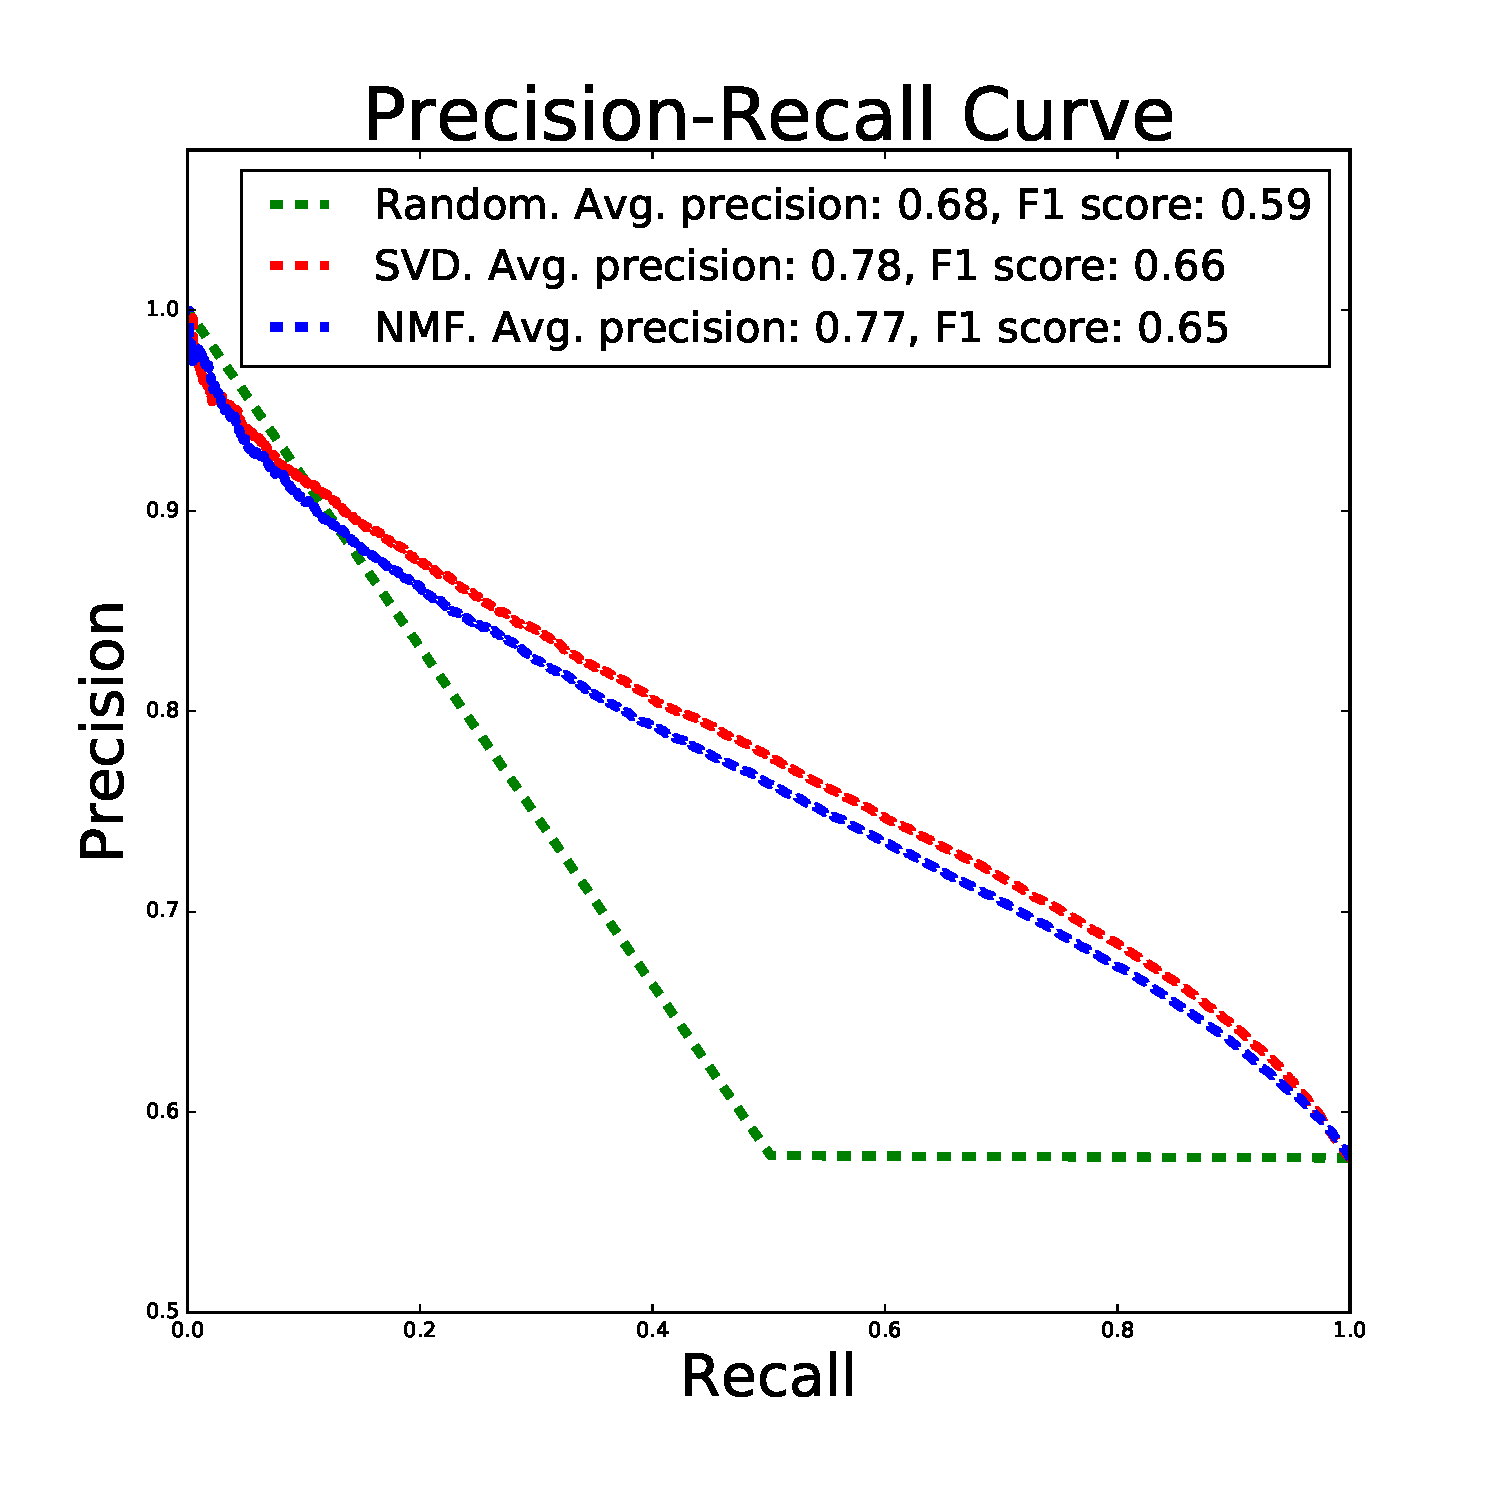
\includegraphics{figures/precision_recall_curve.pdf} \\
\end{tabular}
}
\caption{Matrix Factorization Results: (a) ROC Curve, (b) Precision Recall Curve}
\label{fig:matrixcurves}  
\end{figure*}


To evaluate our prediction performance for the neighbourhood models, we used two accepted metrics: one is RMSE, which was used in the \textit{Netflix Prize} competition, and the the winner, Yehuda Koren, demonstrated later in a different paper that RMSE is a good measurment for recommender systems providing "top K recommendations"~\cite{koren2008factorization}. They witnessed that small improvements in the RMSE translated into significant improvments in the quality of the top K items in the recommended list. The scond metric is called Normalized discounted cumulative gain (NDCG), and it is used in many recommendation system studies to score the relevance of the top K items in the list. This metric allows the relvance scores of the items to be real numbers, so we have used our predicted ratings to sort the recommended movie list. The algorithm we used was implemented by Mathieu Blondel~\cite{letorMetrics}. We calculated NDCG@k for $k=\{5, 10, 15, 20\}$, since these numbers represent a reasonable length of movie recommendation list. Most users will find it difficult to pay attention to lists with too many items. 

We present the results of ratings prediction using cosine similarity in the form of RMSE, veraged on the 10-folds cross validation runs, or each of the representative 10 users individually. The RMSE is plotted as a function of  the number of similar users we have taken into account in the prediction. We can see in Figure~\ref{} that \hl{TODO}.
The results of ratings prediction using K-means clustering are presented in the form of NDCG@k averaged on the 10-folds cross validation runs, for each of the representative 10 users individually. For two users we have less than 100 ratings so each cross-validation run resulted in less than 10 ranked reviews; therefore, we report only NDCG@k, k=5 for those users. In Figure\ref{fig:ndcg} the NDCG@k is plotted for each user, when the users are sorted according to three different features: \blackone The number of user ratings \blacktwo The average of user ratings \blackthree The standard deviation of the user ratings. \hl{TODO: figure description}